\documentclass[10pt]{beamer}

\usetheme[progressbar=frametitle]{metropolis}
\usepackage{appendixnumberbeamer}

\usepackage{booktabs}
\usepackage[scale=2]{ccicons}

\usepackage{pgfplots}
\usepgfplotslibrary{dateplot}

\usepackage{xspace}
\newcommand{\themename}{\textbf{\textsc{metropolis}}\xspace}

\usepackage{graphicx,color}
\usepackage{hyperref}
\usepackage{url}
\usepackage{booktabs}
\usepackage{amsfonts}
\usepackage{nicefrac}
\usepackage{microtype}
\usepackage{bbm}

\usepackage{amsmath, amsfonts, amssymb}
\newtheorem{assumption}{Assumption}
\usepackage{mathtools}
\usepackage{graphicx}
\usepackage{bm}

\usepackage{physics}

\usepackage{algorithm}
\usepackage{algpseudocode}

\definecolor{oxfordnavy}{HTML}{0B1026}
\definecolor{hotpink}{HTML}{FF4FD8}

% Common shortcuts
\def\mbb#1{\mathbb{#1}}
\def\mfk#1{\mathfrak{#1}}

\def\bN{\mbb{N}}
\def \C{\mbb{C}}
\def \R{\mbb{R}}
\def\bQ{\mbb{Q}}
\def\bZ{\mbb{Z}}
\def \cph{\varphi}
\renewcommand{\th}{\theta}
\def \ve{\varepsilon}
\newcommand{\mg}[1]{\| #1 \|}

% Often helpful macros
\newcommand{\floor}[1]{\left\lfloor#1\right\rfloor}
\newcommand{\ceil}[1]{\left\lceil#1\right\rceil}
\renewcommand{\P}{\mathbb P\qty}
\newcommand{\E}{\mathbb{E}\qty}
\newcommand{\Et}{\mathbb{E}_{\mathcal F_{t-1}} \qty}
\newcommand{\Pt}{\mathbb{P}_{\mathcal F_{t-1}} \qty}
\newcommand{\Cov}{\mathrm{Cov}\qty}
\newcommand{\Var}{\mathrm{Var}\qty}

\newcommand{\lr}{\mathrm{lr}}
\renewcommand{\grad}{\nabla} 
\newcommand{\1}{\mathbbm{1}}

% Sets
\usepackage{braket}

\graphicspath{{/}}
\usepackage{float}

\renewcommand{\set}[1]{\left\{#1\right\}}
\newcommand{\given}{\;\middle|\;}

\title{EGGROLL Scaling}
\date{\today}
\author{Rohan Mukherjee}
\institute{University of Oxford}
%\titlegraphic{\hfill
\includegraphics[height=2cm]{logo.png}}

\begin{document}

\maketitle

\begin{frame}{Table of Contents}
  \setbeamertemplate{section in toc}[sections numbered]
  \tableofcontents[hideallsubsections]
\end{frame}

\section{Motivation}

\subsection{Preliminaries}
\begin{frame}{The Problem}
    \begin{definition}[]
    A function $f: \R^d \to \R$ is called $L$-smooth if 
    \begin{align*}
        \| \grad f(x) - \grad f(y) \| \leq L \| x-y \|.
    \end{align*}    
    \end{definition}

    \begin{definition}[]
        A function $f: \R^d \to \R$ is called $\rho$-Hessian lipschitz if
        \begin{align*}
            \| \grad^2 f(x) - \grad^2 f(y) \|_2 \leq \rho \|x-y \|
        \end{align*}
    \end{definition}

    \begin{block}{Main Goal}
    \[
    \min_{x\in\mathbb{R}^d} f(x) 
    \]
    One problem: Even verifying if $x \in \R^d$ is a local minimum is NP-hard. 
    \end{block}
\end{frame}

\begin{frame}{Stationary Points}
    Instead, we want to find stationary points:
    \begin{definition}[]
        A point $x \in \R^{d}$ is an $\ve$-first order stationary point if 
        \begin{align*}
            \mg{\grad f(x)} \leq \ve.
        \end{align*}
    \end{definition}
    \begin{definition}[]
        When $f$ is $\rho$-Hessian Lipschitz, a point $x \in \R^d$ is an $\ve$-second-order stationary point if 
        \begin{align*}
            \mg{\grad f(x)} \leq \ve , \quad \grad^2 f(x) \succeq -\sqrt{\rho \ve} I.
        \end{align*}
        Best you can (reasonably*) hope for: SOSP.
    \end{definition}
\end{frame}

\begin{frame}{Gradient Descent}
    \begin{algorithm}[H]
\caption{Gradient Descent}
\label{alg:gradient-descent}
\begin{algorithmic}[1]
    \Require Initial point $x_0 \in \mathbb{R}^d$,
             number of iterations $T$
    \For{$k = 0,1,\ldots,T-1$}
        \State $x_{k+1} \gets x_k - \frac 1L \nabla f(x_k)$
    \EndFor
    \State \Return $x_T$
\end{algorithmic}
\end{algorithm}

\begin{theorem}[]
    In $T = O(L(f(x_0) - f^*) / \ve^2)$ iterations, $x_T$ is a FOSP.
\end{theorem}
\end{frame}

\begin{frame}{Why Gradient Free?}
    \begin{itemize}
    \item In many applications (e.g., RL), gradients are difficult or impossible to compute
    \item Instead, we may only have access to function evaluations
    \item \textbf{Question:} Can we efficiently optimize $f$ using only zeroth-order information?
\end{itemize}
\end{frame}

\subsection{Previous Work}
\begin{frame}{Zero-Order Methods}
    The main idea is to use the gradient estimator
    \begin{align*}
        \tilde \grad f(x) \coloneqq \frac{f(x + \sigma p) - f(x - \sigma p)}{2\sigma} p, \quad p \sim \mathcal N(0,I_d)
    \end{align*}
    For $L$-smooth non-convex $f$, in $T = O(d/\ve^2)$ iterations \cite{ghadimi2013stochastic} \cite{nesterov2017random}
    \begin{align*}
        \min_{t \leq T} \E(\| \grad f(x_t) \| ) \leq \ve
    \end{align*}
    Typically, zero-order methods take $d$ times more iterations than first order ones
\end{frame} 

\begin{frame}{Common Problem}
    \begin{itemize}
        \item The common problem with all existing ZO literature: requires $p \sim N(0, I_d)$ 
        \item But for ML, $d$ is way too big for this to be tractable
    \end{itemize}
\end{frame}

\section{EGGROLL}
\subsection{Algorithm}
\begin{frame}{Enter: EGGROLL}
    \begin{definition}[Symmetric EGGROLL Update]
        With $a_i \overset{i.i.d.}{\sim} \mathcal N(0, I_d)$, $b_i \overset{i.i.d.}{\sim} \mathcal N(0, I_m)$ and $P_i = a_ib_i^\top$,
        \begin{align*}
            g_\sigma^{r}(X) \coloneqq \frac 1r \sum_{i=1}^r \frac{f(X + \sigma P_{i}) - f(X - \sigma P_{i})}{2\sigma} P_{i}
        \end{align*}
    \end{definition}

    \begin{algorithm}[H]
    \caption{Rank-\(r\) Symmetric EGGROLL}
    \label{alg:symmetric-eggroll}
    \begin{algorithmic}
        \Require Initial point \(X_0 \in \mathbb R^{d\times m}\), horizon \(T\), stepsize \(\eta>0\), smoothing radius \(\sigma>0\), rank \(r\in \mathbb N\)
        \For{\(t = 0,\ldots,T-1\)}
            \State Sample $\set{a_{t,i}}_{i=1}^r \sim \mathcal N(0,I_d)$ and $\set{b_{t,i}}_{i=1}^r \sim \mathcal N(0,I_m)$
                
            \State Update $X_{t+1}
                \gets
                X_t-\eta g_\sigma^r(X_t)$
        \EndFor
        \State \Return \(X_T\)
    \end{algorithmic}
    \end{algorithm}
\end{frame}

\subsection{Convergence}
\begin{frame}{Main Theorem (informal)}
    \begin{theorem}
        Consider running Algorithm~\ref{alg:symmetric-eggroll}. Suppose $0 < \delta \leq 1/e$. Suppose
        \begin{align*}
            \sigma = \tilde{O}\qty(\frac{\ve}{dm\sqrt{r}L}), \quad \eta = \tilde{O}\qty(\frac{r^2}{dmL}).
        \end{align*}
        Then in
        \begin{align*}
            T = \tilde{O}\qty(\frac{dm}{r} \cdot \frac{L(f(X_0) - f^*)}{\ve^2})
        \end{align*}
        iterations (with each iteration using $2r$ function evaluations), with probability at least $1-\delta$, at least $3/4$ of the iterates are $\ve$-first order stationary points. 
    \end{theorem}
\end{frame}

\begin{frame}{Things to bound}
    From $L$-smooth you get 
    \begin{align*}
        f(x+h) \leq f(x) + \langle \grad f(x) , h \rangle + \frac{L}{2} \mg{h}^2
    \end{align*}
    By using $ab \leq (a^2+b^2)/2$ and $\mg{a+b}^2 \leq 2\mg{a}^2 + 2\mg{b}^2$ a few times,
    \begin{align*}
        f(X_{t+1}) - f(X_t) &\leq -\frac{\eta}{2r} \sum_{i=1}^r |\langle \grad f(X_t), P_{t,i} \rangle|^2 + \frac{\eta \sigma^2 L^2}{2r} \sum_{i=1}^r \mg{P_{t,i}}^4 \\
        &\quad + L\eta^2 \left \| \frac{1}{r} \sum_{i=1}^r  \langle \grad f(X_t), P_{t,i} \rangle P_{t,i} \right\|^2 + \frac{\eta^2 L^3 \sigma^2}{r} \sum_{i=1}^r \mg{P_{t,i}}^6
    \end{align*}
\end{frame}

\subsubsection{Square Error Term}
\begin{frame}{Subgaussian}
    To bound \begin{align*}
        \left \| \frac{1}{r} \sum_{i=1}^r  \langle \grad f(X_t), P_{t,i} \rangle P_{t,i} \right\|^2
    \end{align*}
    we will show it is ``subgaussian enough''.  
    \begin{definition}[Subgaussian distribution]
    Random variable $X$ is said to be $SG(\sigma)$ if
    \begin{align*}
        \E[\exp(X^2/\sigma^2)] \leq 2
    \end{align*} 
    and $nSG(\sigma)$ if
    \begin{align*}
        \E[\exp(\mg{X}^2/\sigma^2)] \leq 2
    \end{align*}   
    \end{definition}
    As an example $Z \sim \mathcal N(0,I)$ is $nSG(c\sqrt{d})$.
\end{frame}

\begin{frame}{Concentration Lemma}
    \begin{lemma}[\cite{jin2019short}]
        Let random vectors $x_1, \ldots, x_n \in \R^d$, and corresponding filtrations $\mathcal F_t = \sigma(x_1, \ldots, x_t)$ satisfy that 
        \begin{align*}
            \Et[x_t] = 0, \quad \Pt(\mg{x_t} \geq s) \leq 2e^{-\frac{s^2}{2\sigma^2}} \quad \forall s \in \R
        \end{align*}
        Then there exists an absolute constant $c$ such for any fixed $\delta > 0, \theta > 0$, with probability at least $1-\delta$,
        \begin{align*}
            \left\|\sum_{i=1}^n x_i\right\| \leq c\cdot \theta \sum_{i=1}^n \sigma_i^2 + \frac{1}{\theta} \log(\frac{2d}{\delta}).
        \end{align*}
\end{lemma}
\end{frame}

\begin{frame}{Main Theorem}
    \begin{theorem}\label{error_concentration}
        Let $\set{\mathcal F_t}_{t \geq -1}$ be a filtration, and let $\set{a_t}_{t \geq 0}, \set{b_t}_{t \geq 0} $ be two sequences of independent random vectors such that $a_t \sim \mathcal N(0, I_d)$, $b_t \sim \mathcal N(0, I_m)$, $a_t, b_t \in \mathcal F_t$ and $a_t, b_t$ are independent of $\mathcal F_{t-1}$. Let $\set{V_t}_{t \geq 0}$ be a sequence of random matrices such that $V_t \in \mathcal F_{t-1}$. For each $\tau \geq 0$, let 
        \begin{align*}
            E_\tau = \sum_{t=0}^{\tau-1} \qty(V_t - \langle V_t, a_tb_t^\top \rangle a_t b_t^\top)
        \end{align*}
        Then, there exists some absolute constants $C > 0, c > 0$ such that for any $\tau \in \bZ^+$, and $0 < \delta < 1/e$, for any $\theta > 0$, with probability at least $1-\delta$ given $\mathcal F_{t-1}$, 
        \begin{align*}
            \left \|E_{\tau} \right \|_F \leq c \cdot \theta \sum_{t=0}^{\tau-1} dm \log^{3}\qty(\frac{C\tau m}{\delta}) \mg{V_t}_F^2 + \frac{1}{\theta} \log(\frac{Cm^2d \tau}{\delta}).
        \end{align*}
    \end{theorem}
\end{frame}

\begin{frame}{Proof Idea}
    \begin{lemma}
        Let $X$ follow $\chi^2_d$ distribution and $0 < \delta < 1/e$. Then there exists $L_{\delta}$ such that for every $d$, with
        \begin{align*}
            A \coloneqq \set{dL_{\delta}^2 \leq X \leq 3d\log(C/\delta)}
        \end{align*}
        we have
        \begin{align*}
            \E[(X-d) ; A] = 0, \quad \P(A) \geq 1-\delta
        \end{align*}
        for some absolute constant $C$.
    \end{lemma}
\end{frame}

\begin{frame}{Proof of Main Theorem I}
    \begin{block}{Proof}
    \begin{itemize}
        \item The main trick is to use SVD of $V_t = P \Sigma Q^\top$
        \item By previous lemma, can define event $A_t \cap B_t$ where all $\mg{a_t} \leq \sqrt{3d \log(\cdot)}$ and $|b_t^\top q_i| \leq \sqrt{3 \log(\cdot)}$ whp.
        \item Most crucially, $b_t^\top q_i$ are independent as $q_i$ are orthogonal.
        \item Then $R_t = (V_t - \langle V_t, a_tb_t^\top \rangle a_t b_t^\top)\1_{A_t \cap B_t}$ is mean 0. (**)
        \item This is done by considering $\Et[Q^\top b_t b_t^\top ; B_t]$.
        \end{itemize}
        \end{block}
    \end{frame}
    \begin{frame}{Proof of Main Theorem II}
        \begin{itemize}
        \item $\mg{aa^\top V bb^\top}_F \leq |a^\top V b| \sqrt{9md \log(\cdot)}$ on $A_t \cap B_t$
        \item Given $b$, $a^\top V b \sim \mathcal N(0, \mg{Vb}^2)$
        \item Then $\E[\exp(t(a^\top Vb)^2) \mid b] \leq \exp(2t \mg{Vb}^2)$
        \item As $Vb \sim \mathcal N(0, VV^\top)$, $\E[\exp(2t \mg{Vb}^2)] \leq \exp(4t \mg{V}_F^2)$
        \item Yields $R_t$ is $\tilde O(md \mg{V}_F^2)$ subgaussian.
        \item Utilizing lemma from before, we are done. \qed
    \end{itemize}
\end{frame}

\subsubsection{Descent}
\begin{frame}{Descent}
    The rest of the proof is in showing 
        \begin{align*}
        \sum_{t=0}^{\tau-1} \frac 1r \sum_{i=1}^r |\langle \grad f(X_t), P_{t,i} \rangle|^2 \geq \tilde \Omega \qty(\sum_{t=0}^{\tau-1} \mg{\grad f(X_t)})
    \end{align*}

\begin{itemize}
    \item Since $\E[|\langle \grad f(X_t), a_tb_t^\top \rangle |^2] = \| \grad f(X_t)\|_F^2$, know at least once every $t_f(\delta) = \frac{1}{r} \log(\cdot)$ iterations, $\frac 1r \sum_{i=1}^r |\langle \grad f(X_t), P_{t,i} \rangle|^2 \geq \frac 12 \mg{\grad f(X_t)}_F^2$
    \item $\eta$ and $\sigma$ tuned so that on intervals of length $t_f(\delta)$, $|\grad f(X_t)|$ does not change by more than factor of 4
    \item Thus with just one $t$ with $\frac 1r \sum_{i=1}^r |\langle \grad f(X_t), P_{t,i} \rangle|^2 \geq \frac 12 \mg{\grad f(X_t)}^2$, can replace with the sum (up to log factors)
    \item Which completes the proof. \qed
\end{itemize}
\end{frame}

\section{Scaling}
\subsection{Random projections}
\begin{frame}{r-Dimensional Random Projection}
    EGGROLL update:
    \begin{align*}
        \frac 1r \left(\sum_{i=1}^r P_iP_i^\top \right) \grad f(x)
    \end{align*}
    Let $\Pi_Q$ be the matrix which projects onto the uniformly random r-dimensional subspace $Q$. Then by rotational invariance
    \begin{align*}
        \E[\Pi_Q] = cI
    \end{align*}
    Taking traces $\Tr(P_Q) = r$ and $\Tr(I) = d$, so $c = r/d$. Therefore,
    \begin{align*}
        \E[\|\Pi_Q g \|^2] = \E[\langle g, \Pi_Q g \rangle] = \langle g, \E[\Pi_Q] g \rangle = \frac{r}{d} \mg{g}^2
    \end{align*}
    So every iteration, we can only really capture $r/d$ fraction of the available descent.
\end{frame}

\begin{frame}{Towards Improvement}
    \begin{itemize}
        \item Naturally, to escape $\E[\mg{\Pi_Q g}^2] = \frac{r}{d} \mg{g}^2$, need better directions. 
        \item For $L$-smooth convex functions, have co-coercivity inequality
        \begin{align*}
            \langle \grad f(y) - \grad f(x), y-x \rangle \geq \frac{1}{L} \mg{y-x}^2
        \end{align*}
        When $y = x^+$ the next iterate in GD, get
        \begin{align*}
            \langle \grad f(x^+), \grad f(x) \rangle \geq \mg{\grad f(x^+)}^2
        \end{align*}
        \item Suggests, if we know which perturbations are well-aligned with $\grad f(x)$, maybe they will also be with $\grad f(x^+)$!
        \item Non-convex function is (nearly) convex around a local min.
        \item \alert{Open question: Other ideas?}
    \end{itemize}
\end{frame}

\section{Future Directions}
\subsection{Saddle Escape}
\begin{frame}{Hessian Escape}
\begin{algorithm}[H]
\caption{Perturbed Gradient Descent}
\begin{algorithmic}[1]
\Require Initial point $x_0$, step size $\eta$, perturbation radius $r$
\For{$t=0,1,2,\dots$}
    \If{perturbation condition holds}
        \State Sample $\xi_t \sim \mathrm{Unif}(B_0(r))$
        \State $x_t \gets x_t+\xi_t$
    \EndIf
    \State $x_{t+1}\gets x_t-\eta\nabla f(x_t)$
\EndFor
\end{algorithmic}
\end{algorithm}
\begin{theorem}[\cite{jin2017escape}]
    PGD converges to SOSP in $T = O\left(\frac{L (f(x_0)-f^*)}{\ve^2}\right)$ iterations.
\end{theorem}
\end{frame}

\begin{frame}{Perturbed Gradient Descent}
    Consider quadratic $f(x) = x^\top H x$, with $H = \mathrm{diag}(-1, 1, \ldots, 1)$

    Then $x_t = x_{t-1} - \eta \grad f(x_{t-1}) = (I- \eta H)^t x_0$

    Then with $\lambda_i = \lambda_i(H)$ and $\alpha_i = e_i^\top x_0$,
    \begin{align*}
        f(x_t) - f(x_0) = \sum_{i=1}^d \lambda_i (1-\eta \lambda_i)^{2t} \alpha_i^2 \leq -1.5^{2t} \alpha_1^2 + 0.5^{2t}
    \end{align*}
    When $x_0 \sim \mathrm{Unif}(B_0(1))$, whp $\alpha_1^2 = \Omega(\delta^2/d)$. Thus takes $\log(\sqrt{d}/\delta)$ steps for decrease by constant amount.

    \begin{center}
        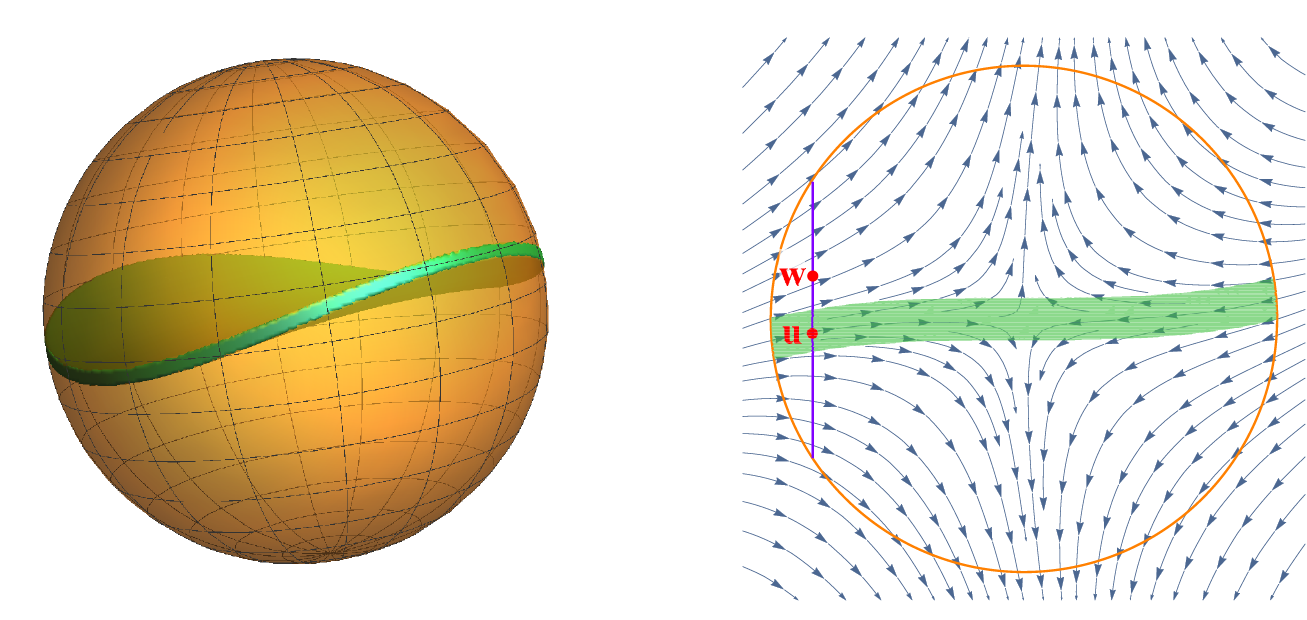
\includegraphics[width=0.55\textwidth]{flow.png}
    \end{center}
\end{frame}

\begin{frame}{Zero-Order PGD}
    \begin{algorithm}[H]
\caption{Perturbed Zeroth-Order Gradient Descent}
\begin{algorithmic}[1]
\Require Initial point $x_0$, horizon $T$, step size $\eta$, smoothing radius $u$, perturbation radius $r$, batch size $m$
\For{$t=0,1,\dots,T-1$}
    \State Sample $Z_{t,1},\dots,Z_{t,m}\overset{\mathrm{i.i.d.}}{\sim}\mathcal N(0,I_d)$
    \State $g_u^{(m)}(x_t)
        \gets
        \frac{1}{m}\sum_{i=1}^m
        \frac{f(x_t+uZ_{t,i})-f(x_t-uZ_{t,i})}{2u}
        Z_{t,i}$
    \State Sample $Y_t\sim \mathcal N\left(0,r^2/d \cdot I_d\right)$
    \State $x_{t+1}\gets x_t-\eta\left(g_u^{(m)}(x_t)+Y_t\right)$
\EndFor
\State \Return $x_{T}$
\end{algorithmic}
\end{algorithm}
\begin{theorem}[\cite{ren2023escaping}]
    Perturbed zeroth-order GD converges to $\ve$-SOSP in time 
    \begin{align*}
        T = O\left(\frac{d}{m} \cdot \frac{(L+L^2)\rho^{3/2} (f(x_0)-f^*)}{\ve^{5/2}}\right)
    \end{align*}
\end{theorem}
\end{frame}

\subsection{Linear Coupling and Accelerated Methods}
\begin{frame}{Nesterov AGD}
    \begin{algorithm}[H]
\caption{Nesterov Accelerated Gradient Descent}
\begin{algorithmic}[1]
\Require Initial point $x_0 \in \mathbb{R}^d$, smoothness $L$, iterations $T$
\State $y_0 \gets x_0$
\For{$k = 1,2,\dots,T$}
    \State $x_k \gets y_{k-1} - \eta \grad f(y_{k-1})$ 
    \State $y_k \gets x_k + \frac{k-1}{k+2} (x_k -x_{k-1})$
\EndFor
\State \Return $x_{T+1}$
\end{algorithmic}
\end{algorithm}
\begin{theorem}[]
    For any $\eta \leq 1/L$, Nesterov AGD has 
    \begin{align*}
        f(x_T) - f^* \leq O\qty(\frac{L\mg{x_0-x^*}^2}{T^2})
    \end{align*}
\end{theorem}
Proved using the Lyapunov $A_k(f(x_k) - f^*) + \frac 12 \mg{z_k-x^*}^2$
\end{frame}
\begin{frame}{ODE View of Acceleration}
    In \cite{su2016differential} they model Nesterov's AGD using a second-order ODE. By taking step size $s \to 0$ get that $X$ satisfies
    \begin{align*}
        \ddot{X} + \frac{3}{t} \dot{X} + \grad f(X) = 0.
    \end{align*}
    Taking inner product with $\dot{X}$,
    \begin{align*}
        \dv{t} (\frac12 \mg{\dot{X}}^2 + f(X)) = -\frac{3}{t} \mg{\dot{X}}^2
    \end{align*}
    Motivated by this, in \cite{jin2017accelerated} they use the Hamiltonian $E_t = f(x_t) + \frac{1}{2\eta} \mg{v_t}$ to show perturbed AGD escapes saddle points faster than perturbed GD:
    \begin{theorem}[]
        w.p. at least $1-\delta$, Perturbed AGD converges to SOSP in time
        \begin{align*}
            T = \tilde{O} \left(\frac{L^{1/2} \rho^{1/4} (f(x_0) - f^*)}{\ve^{7/4}} \right)
        \end{align*}
    \end{theorem}
\end{frame}

\subsection{Linear Coupling}
\begin{frame}{Mirror Descent}
    Problem: gradient descent makes no attempt to characterise lower bound on $f^*$. For any points $x_0, \ldots, x_T$, by convexity
    \begin{align*}
        \forall u \quad f(u) \geq \frac{1}{T} \sum_{t=0}^{T-1} f(x_t) + \frac 1T \sum_{t=0}^{T-1} \langle \grad f(x_t), u-x_t \rangle
    \end{align*}
    And so,
    \begin{align*}
        f(\bar x) - f(u) \leq \frac{1}{T} \sum_{t=0}^{T-1} \langle \grad f(x_t), x_t-u \rangle \eqqcolon R_T(u)
    \end{align*}
    Considering a regularized version
    \begin{align*}
        \widetilde{R_T}(u) \coloneqq \frac{1}{T} \left(-\frac{w(u)}{\alpha} + \sum_{t=0}^{T-1} \langle \grad f(x_t), x_t-u \rangle \right)
    \end{align*}
    By choosing $x^+ = \mathrm{argmax}_u \widetilde{R_k}(u)$, MD converges in $T = O(\rho^2 / \ve^2)$ iterations where $\rho^2$ is the average value of $\mg{\grad f(x_t)}_*^2$
\end{frame}
\begin{frame}{MD Definitions}
    \begin{definition}[]
        For closed and convex $Q \subset \R^d$, $w: Q \to \R$ is a DGF if $w$ is 1-strongly convex wrt $\mg{\cdot}$. The Bregman divergence is defined as
        \begin{align*}
            V_x(y) = w(y) - \langle \grad w(x), y-x \rangle - w(x)
        \end{align*}
        The properties of DGF ensures $V_x(x) = 0$ and $V_x(y) \geq \frac12 \mg{x-y}^2 \geq 0$.
    \end{definition}
    
    
    \begin{block}{Examples}
        \begin{itemize}
            \item $w(y) = \frac 12 \mg{y}_2^2$ for the $\ell^2$ norm gives $V_x(y) = \frac12 \mg{x-y}^2$
            \item When $Q = \Delta$ is the probability simplex, $w(y) = \sum_i y_i \log(y_i)$ for the $\ell^1$ norm gives $V_x(y) = \sum_i y_i \log(y_i/x_i)$ 
        \end{itemize}
    \end{block}
    \begin{definition}[]
        The mirror descent update step with step length $\alpha$ 
        \begin{align*}
            x^+ = \mathrm{Mirr}_x(\alpha \grad f(x)), \; \mathrm{Mirr}_x(\xi) = \mathrm{argmin}_{y \in Q} \set{V_x(y) + \langle  \xi, y-x \rangle}
        \end{align*}
    \end{definition}
\end{frame}

\begin{frame}{MD Core Lemma}
    \begin{lemma}[\cite{allenZhu2016linear}] 
        For all $u \in Q$,
        \begin{align*}
            \alpha (f(x) - f(u)) \leq \alpha \langle \grad f(x), x-u \rangle \leq \frac{\alpha^2}{2} \mg{\grad f(x)}^2_* + V_x(u) - V_{x^+}(u)
        \end{align*}
    \end{lemma}
    \begin{theorem}[]
        Where $\Theta \geq V_{x_0}(x^*)$, by telescoping the previous lemma, MD has $f(\bar x) - f^* \leq \ve$ in time
        \begin{align*}
            T = O\left(\frac{2\Theta L^2}{\ve^2}\right)
        \end{align*}
    \end{theorem}
\end{frame}
\begin{frame}{Linear Coupling}
    The big question: Can GD and MD be combined for faster methods?

    GD tells us to go one place, while MD tells us to go another. Where should we go?
    \begin{align*}
        x_{k+1} &= \tau z_k + (1-\tau) y_k \\
        y_{k+1} &= \mathrm{Grad}(x_{k+1})\\
        z_{k+1} &= \mathrm{Mirr}_{z_k}(\alpha \grad f(x_{k+1}))
    \end{align*}
    The answer: a linear combination!
\end{frame}

\begin{frame}{Convergence}
    \begin{lemma}[Coupling]
        When $\tau \in (0,1)$ satisfying $ \frac{1-\tau}{\tau} = \alpha L$, for all $u \in Q$, \begin{align*}
         \alpha \langle \grad f(x_{k+1}), x_{k+1}-u \rangle \leq \alpha^2 L(f(y_k) - f(y_{k+1})) + V_{z_k}(u) - V_{z_{k+1}}(u)
        \end{align*}
    \end{lemma}
    \begin{theorem}[]
        Telescoping the previous lemma,
        \begin{align*}
            \alpha T(f(\bar x) - f(x^*)) \leq \alpha^2 L(f(y_0) - f(y_T)) + V_{x_0}(x^*) - V_{x_T}(x^*)
        \end{align*}
        Choosing $\alpha = \sqrt{\Theta/L\ve}$, and restarting the procedure a few times, obtain $\ve$-approx. solution in 
        \begin{align*}
            T = O(\sqrt{L\Theta/\ve} + \sqrt{L\Theta/2\ve} + \cdots) = O(\sqrt{L\Theta/\ve})
        \end{align*}
        matching Nesterov AGD.
    \end{theorem}
\end{frame}

\begin{frame}{Open Question}
    \begin{itemize}
        \item Experiments show replacing $\grad f(x)$ with the EGGROLL approximation, MD still converges.
        \item The proof would likely give the tools to design an accelerated ZO method by linear mixing of GD and MD.
        \item Problem: EGGROLL update only gives lower bound on a random $r$-dimensional (affine) subspace $x_t + Q_t$ each iteration.
        \item First idea: average projection
        \begin{align*}
            \frac{d}{r} \cdot \frac{1}{T} \sum_{t=0}^{T-1} \Pi_{x_t + Q_t} x^* \approx x^* ?
        \end{align*}
        \item This has huge variance. 
    \end{itemize}
\end{frame}

\subsection{Variance Reduction}
\begin{frame}{Variance Reduction}
    Consider the problem
    \begin{align*}
        \min_x f(x) \coloneqq \frac 1n \sum_{i=1}^n f_i(x)
    \end{align*}
    where each $f_i$ is $L$-smooth.

    SGD chooses $i \sim \mathrm{Unif}([n])$ and applies an update
    \begin{align*}
        x^+ = x - \eta \grad f_i(x)
    \end{align*}
    Problem: this has huge variance
    \begin{align*}
        \frac{1}{n} \sum_{i=1}^n \mg{\grad f_i(x) - \grad f(x)}^2
    \end{align*}
\end{frame}

\begin{frame}{Variance Reduction}
    However, if you know the full gradient at a snapshot point $\tilde x$, $\grad f(\tilde x)$, you can compute
    \begin{align*}
        v_t = \grad f_i(x_t) - \grad f_i(\tilde x) + \grad f(\tilde x)
    \end{align*}
    Which has variance
    \begin{align*}
        \Var(v_t) \leq O(\mg{x_t - \tilde x}^2)
    \end{align*}

    Then by infrequently computing the full gradient and linearly coupling three points $x_{k+1} = \tau_1 z_k + \tau_2 \tilde x + (1-\tau_2 - \tau_1) y_k$,
    \begin{theorem}
        The algorithm in \cite{allenZhu2016variance} produces an $\ve$-FOSP in only 
        \begin{align*}
            O\left(\frac{n^{2/3}L(f(x_0) - f(x^*))}{\ve^2}\right)
            \end{align*}
            which beats GD and SGD by $n^{1/3}$.
        \end{theorem}
\end{frame}

\begin{frame}{EGGROLL Variance Reduction}
    \begin{itemize}
        \item For EGGROLL, maybe infrequently compute a full gradient
        \item Could get lower variance for gradient estimator 
        \item By linearly coupling so the points stay close, might exploit more descent
        \item Potentially speeding up convergence.
    \end{itemize}
\end{frame}

{
\setbeamercolor{palette primary}{fg=hotpink, bg=oxfordnavy}
\begin{frame}[standout]
  Questions?
\end{frame}
}

\section{References}
\begin{frame}[allowframebreaks]{References}

  \bibliographystyle{abbrv}
  \bibliography{references}

\end{frame}

\end{document}
